%\documentclass[fleqn]{report}
%\usepackage{graphicx} % om PostScript plaatje in te lassen
%\usepackage{here}     % voor geforceerde plaatsing figuren
%\usepackage{amsmath}
%\textwidth=17.0cm
%\textheight=22.0cm
%\topmargin=-1cm
%\oddsidemargin=-0.3cm
%\evensidemargin=-0.3cm
%
%%packages
%\usepackage{amsmath}
%\usepackage{cite}
%\usepackage[toc,page]{appendix}
%\usepackage{fancyvrb}
%\usepackage{tikz}
%\usepackage{multicol}
%\usepackage{framed}
%\usepackage{pgfplots}
%%\usepgfplotslibrary{fillbetween}
%\usepackage{fixltx2e}
%\usepackage{subfigure}
%\usepackage{lscape}
%\usepackage{enumitem}
%\usepackage{filecontents}
%\usetikzlibrary{decorations.pathmorphing}
%\usepackage{lmodern}
%\usepackage{pgfplotstable}
%
%\usetikzlibrary{arrows}
%%\usetikzlibrary{arrows.meta}
%
%
%
%\usetikzlibrary{decorations.pathreplacing,decorations.markings,snakes}
%
%%tikz labraries
%\usetikzlibrary{matrix}
%\usetikzlibrary{decorations.pathreplacing}
%\usetikzlibrary{positioning}
%\usetikzlibrary{calc}
%\usetikzlibrary{shapes,arrows, chains}
%\usetikzlibrary{patterns}
%
%\usetikzlibrary{intersections}
%\usetikzlibrary{decorations.markings}
%\usetikzlibrary{calc,intersections}
%%\usetikzlibrary{decorations.pathreplacing,bending}
%
%%extra instellingen
%\newlist{aims}{enumerate}{1}
%\setlist[aims,1]{
%  label={*},
%  leftmargin=*,
%  align=left,
%  labelsep=2mm,
%}
%
%\newlist{aims2}{enumerate}{1}
%\setlist[aims2,1]{
%  label={},
%  leftmargin=0pt,
%  align=left,
%  labelsep=4mm,
%}
%
%\newlist{aims3}{enumerate}{1}
%\setlist[aims3,1]{
%  label={-},
%  leftmargin=2cm,
%  align=left,
%  labelsep=0.4mm,
%}
%
%\usepackage{pgfplots}
%
%\begin{document}


\begin{tikzpicture}[scale=2]
\small 
\node [above right] (Nederland) at (0,0) {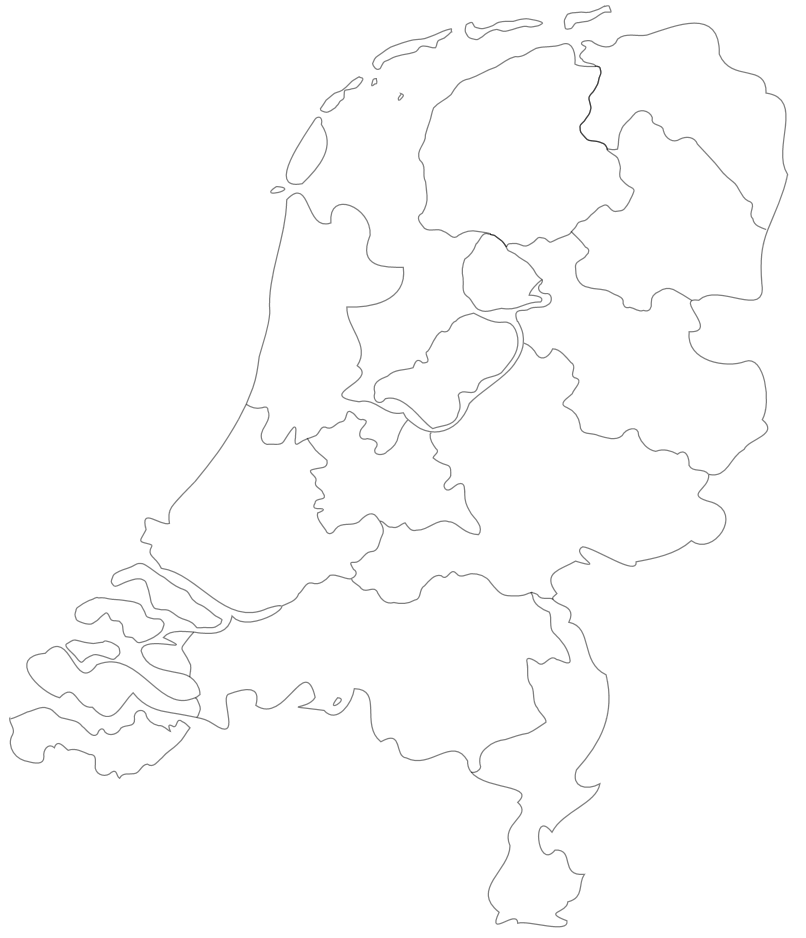
\includegraphics[height=4cm]{tikz/images/Nederland}};
\begin{scope}

\coordinate (schiphol) at (0.7,1.2);
\coordinate (vlissingen) at (0.15,0.57);
\coordinate (eindhoven) at (1,0.52);
%\coordinate (debilt) at (0.85, 1.0);

%\node [above](Eindhoven) at (eindhoven) {Eindhoven};
\node [above](Schiphol) at (schiphol) {Schiphol Airport};
%\node [above] (Vlissingen) at (vlissingen) {Vlissingen};
%\node [above](Debilt) at (debilt) {De Bilt};

\fill (schiphol) circle (0.2pt);
%\fill (eindhoven) circle (0.2pt);
%\fill (vlissingen) circle (0.2pt);
%\fill (debilt) circle (0.2pt);

\end{scope}



\end{tikzpicture}
%
%\end{document}